% Linvesther — protocol whitepaper. Build: tectonic whitepaper.tex
\documentclass[11pt,a4paper]{article}

\usepackage[margin=2.7cm,top=2.8cm,bottom=2.6cm]{geometry}
\usepackage{fontspec}
\setmainfont{texgyrepagella}[Extension=.otf,UprightFont=*-regular,BoldFont=*-bold,ItalicFont=*-italic,BoldItalicFont=*-bolditalic]
\setsansfont{texgyreheros}[Extension=.otf,UprightFont=*-regular,BoldFont=*-bold,ItalicFont=*-italic,BoldItalicFont=*-bolditalic,Scale=0.96]
\setmonofont{texgyrecursor}[Extension=.otf,UprightFont=*-regular,BoldFont=*-bold,ItalicFont=*-italic,BoldItalicFont=*-bolditalic,Scale=0.9]
\usepackage{unicode-math}
\setmathfont{texgyrepagella-math}[Extension=.otf]
\usepackage{microtype}
\usepackage{xcolor}
\usepackage{amsmath}
\usepackage{booktabs,array,tabularx}
\usepackage{titlesec}
\usepackage{fancyhdr}
\usepackage{enumitem}
\usepackage{tikz}
\usetikzlibrary{arrows.meta,positioning,fit,backgrounds,calc}
\usepackage[hidelinks,pdftitle={Linvesther: verifiable performance, private history},pdfauthor={Linvesther}]{hyperref}
\usepackage{setspace}
\usepackage{needspace}
\setcounter{tocdepth}{1}
\setstretch{1.12}

\definecolor{ink}{HTML}{14150F}
\definecolor{moss}{HTML}{4C6B2E}
\definecolor{lime}{HTML}{D0EDAA}
\definecolor{mute}{HTML}{5A5F52}
\definecolor{paper}{HTML}{F6F4EE}
\definecolor{rule}{HTML}{CFCABC}

\hypersetup{colorlinks=true,linkcolor=moss,urlcolor=moss,citecolor=moss}

\setlength{\parindent}{0pt}
\setlength{\parskip}{0.7em}

\titleformat{\section}{\sffamily\Large\bfseries\color{ink}}{\color{moss}\thesection}{0.8em}{}
\titleformat{\subsection}{\sffamily\large\bfseries\color{ink}}{\color{moss}\thesubsection}{0.7em}{}
\titlespacing*{\section}{0pt}{2.2em}{0.8em}
\titlespacing*{\subsection}{0pt}{1.4em}{0.5em}

\pagestyle{fancy}
\fancyhf{}
\renewcommand{\headrulewidth}{0pt}
\fancyhead[L]{\sffamily\footnotesize\color{mute}Linvesther}
\fancyhead[R]{\sffamily\footnotesize\color{mute}Verifiable performance, private history}
\fancyfoot[C]{\sffamily\footnotesize\color{mute}\thepage}
\fancypagestyle{plain}{\fancyhf{}\fancyfoot[C]{\sffamily\footnotesize\color{mute}\thepage}\renewcommand{\headrulewidth}{0pt}}

\newcommand{\term}[1]{\textit{#1}}
\newenvironment{keypoint}
  {\par\medskip\noindent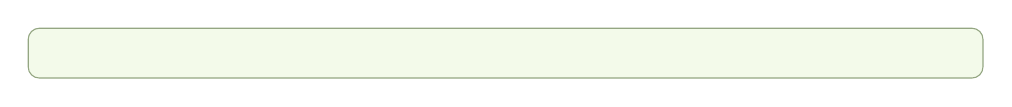
\begin{tikzpicture}\node[draw=moss!60,fill=lime!25,rounded corners=4pt,inner sep=9pt,text width=\dimexpr\linewidth-18pt\relax,align=left]\bgroup\sffamily\small}
  {\egroup;\end{tikzpicture}\par\medskip}

\begin{document}

% ------------------------------------------------------------------ cover
\thispagestyle{empty}
\begin{tikzpicture}[remember picture,overlay]
  \fill[ink] (current page.south west) rectangle (current page.north east);
  \fill[lime] ([xshift=2.7cm,yshift=-4.6cm]current page.north west) rectangle ++(1.1cm,0.09cm);
\end{tikzpicture}
\begin{flushleft}
\color{lime}\sffamily
\vspace*{3.4cm}
{\footnotesize\bfseries\MakeUppercase{Linvesther \quad/\quad Protocol whitepaper}}\\[2.2cm]
{\fontsize{34}{38}\selectfont\bfseries Verifiable performance.\\[0.15em]Private history.}\\[1.4cm]
{\color{paper}\large\begin{minipage}{0.78\textwidth}\setstretch{1.3}
A protocol for turning a trader's real track record into public statements that anyone can check, without ever publishing a balance, a position or a trade.
\end{minipage}}
\vfill
{\color{paper!70!ink}\footnotesize Version 0.1 \quad$\cdot$\quad Draft for public review\\
Networks: Base Sepolia (test network)}
\vspace*{0.8cm}
\end{flushleft}
\newpage

% ------------------------------------------------------------------ abstract
\pagenumbering{roman}
\section*{Abstract}
Financial performance is easy to claim and hard to verify. A screenshot can be edited, a spreadsheet can be curated, and the only way to prove more is to hand over the account itself: balances, positions and every trade. Linvesther proposes a third path. Performance is measured from read-only connections to real accounts, expressed only as ratios, and published as narrow statements that the owner authorizes one by one. Where a stronger guarantee is available, the calculation is proven with a zero-knowledge proof so that anyone can check that a result follows from its inputs without seeing the inputs. Ownership and registration are anchored on a public blockchain, so the record does not depend on the availability or goodwill of any single operator.

This paper describes the technology and the guarantees it provides, as well as the ones it does not. We are deliberate about the second half: a verification system is only as useful as its stated limits.

\vspace{1.2em}
{\small\tableofcontents}
\newpage
\pagenumbering{arabic}

% ------------------------------------------------------------------ 1
\section{The problem}
A track record answers a simple question: \emph{how did this person's money perform, and can I believe it?} Today the answer forces a bad choice.

\textbf{Publish a number, and nothing backs it.} A return figure has a source, a scope, an observation period and a method of calculation. Without them the number cannot be interpreted, and nothing prevents it from being selected after the fact: the best account, the best month, the best window.

\textbf{Publish everything, and lose control.} Sharing the underlying account activity proves more, but it exposes position sizes, strategy, counterparties and net worth. Once disclosed, it cannot be taken back.

Both failures come from the same gap: there is no way to make a \emph{bounded} statement about private data and have others verify it. Linvesther fills that gap. The owner keeps the history; the world receives a statement, its scope, and the evidence that supports it.

% ------------------------------------------------------------------ 2
\section{Design principles}
\begin{description}[leftmargin=1.2em,style=nextline,itemsep=0.4em]
\item[Percentages, never amounts.] Nothing published contains a balance, a position, a trade, an exchange identifier or an absolute amount. Results are ratios computed since the account was connected.
\item[No cherry-picking.] All of an owner's connected accounts are combined into one public record. The owner cannot choose which accounts, or which figures, to show. The only choice is whether the record is public at all.
\item[Consent is exact.] Every disclosure is a specific statement, and the owner's signature covers exactly that statement, its period, its audience and its expiry. Changing any of it invalidates the consent.
\item[Guarantees are separate.] Who provided the data, whether it is complete, whether the calculation is correct, whether it is registered and whether the evidence is available are five different questions. No single badge answers all of them.
\item[No dependence on a vendor.] Registries are public and immutable; the party that submits a transaction can be replaced by anyone, because authority comes from the owner's signature and not from the submitter.
\end{description}

% ------------------------------------------------------------------ 3
\section{System overview}
Figure~\ref{fig:flow} shows how a statement travels from a private account to a public verifier. Everything to the left of the dashed line stays under the owner's control; only what crosses it is public.

\begin{figure}[h]
\centering
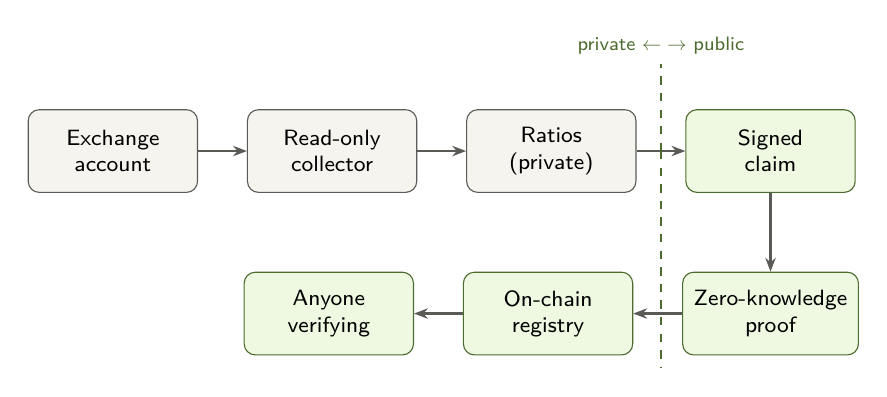
\begin{tikzpicture}[
  node distance=0.5cm and 0.62cm,
  box/.style={draw=ink!70,rounded corners=4pt,fill=white,minimum height=1.05cm,minimum width=2.15cm,align=center,font=\sffamily\footnotesize,inner sep=4pt},
  priv/.style={box,fill=paper},
  pub/.style={box,fill=lime!35,draw=moss},
  arr/.style={-{Stealth[length=5pt]},thick,color=ink!70}
]
\node[priv] (ex) {Exchange\\account};
\node[priv,right=of ex] (col) {Read-only\\collector};
\node[priv,right=of col] (met) {Ratios\\(private)};
\node[pub,right=of met] (clm) {Signed\\claim};
\node[pub,below=1.0cm of clm] (prf) {Zero-knowledge\\proof};
\node[pub,left=of prf] (reg) {On-chain\\registry};
\node[pub,left=of reg] (ver) {Anyone\\verifying};
\draw[arr] (ex)--(col); \draw[arr] (col)--(met); \draw[arr] (met)--(clm);
\draw[arr] (clm)--(prf); \draw[arr] (prf)--(reg); \draw[arr] (reg)--(ver);
\draw[dashed,moss,thick] ($(met.east)!0.5!(clm.west)$) -- ++(0,1.1) node[above,font=\sffamily\scriptsize,color=moss]{private $\leftarrow\;\rightarrow$ public};
\draw[dashed,moss,thick] ($(met.east)!0.5!(clm.west)$) -- ++(0,-2.75);
\end{tikzpicture}
\caption{From a private account to a public, checkable statement.}
\label{fig:flow}
\end{figure}

The remaining sections follow this path: identity and ownership (\S\ref{sec:identity}), measurement (\S\ref{sec:measure}), selective disclosure (\S\ref{sec:claims}), proofs (\S\ref{sec:zk}), the registry (\S\ref{sec:chain}) and finally the trust model (\S\ref{sec:trust}).

% ------------------------------------------------------------------ 4
\section{Identity and ownership}\label{sec:identity}
An identity in Linvesther is a public key, not an account with a company. Two credential types are supported, and both produce the same kind of key.

\textbf{Passkeys.} A device credential based on the WebAuthn standard: the user authenticates with a fingerprint, face or screen lock, and the device signs with an ECDSA key on the P-256 curve. The private key never leaves the device's secure hardware.

\textbf{Password-derived keys.} For users who prefer a password, a P-256 key is generated in the browser and stored only in encrypted form on the user's device, unlocked by the password. The service never sees the password or the key.

To let a blockchain accept these signatures, each identity is represented by a small \term{smart account}: a contract that implements the ERC-1271 standard for validating signatures on behalf of a contract, using the P-256 verification available on the network. The same identity can therefore sign ordinary messages and structured typed data (EIP-712) that any contract can check on-chain.

\textbf{Continuity.} Ownership changes, such as rotating to a new key, follow a two-step lifecycle: the current owner authorizes the change, and it takes effect only once it is confirmed. A requested new owner gains no authority until then. Losing every credential means losing the identity; there is no operator-held backup, by design.

% ------------------------------------------------------------------ 5
\section{Measuring performance}\label{sec:measure}
\subsection{Read-only sources}
Performance is measured from real accounts through read-only connections: exchange API keys restricted to reading, and a read-only report token for brokerage accounts. A connection that carries trading or withdrawal permissions is rejected. The assets always stay at the exchange, and nothing the protocol holds can move them.

\subsection{Time-weighted return}
Deposits and withdrawals must not look like performance. The protocol uses the \term{time-weighted return} (TWR): the period is split at every external cash flow, and the returns of the sub-periods are chained. For a sub-period $j$ with net asset value $V^{\text{start}}_j$ just after the opening flow and $V^{\text{end}}_j$ just before the next one,
\begin{equation}
  r_j = \frac{V^{\text{end}}_j}{V^{\text{start}}_j} - 1,\qquad
  I_j = I_{j-1}\,(1+r_j),\qquad I_0 = 1,
\end{equation}
and the return between two moments $a<b$ is $R[a,b] = I_b/I_a - 1$. A deposit changes the account's value but not the index $I$, so adding capital neither creates nor hides performance. For an account with daily observations $E_t$ and net flow $F_t$ the daily return is $(E_t - F_t)/E_{t-1} - 1$.

\subsection{Risk and consistency}
From the daily returns $r_t$ the protocol derives standard measures, each with a declared minimum sample below which it is reported as \emph{unavailable} rather than guessed:
\begin{align}
  \text{Max drawdown} &= \max_t\Bigl(1 - \frac{I_t}{\max_{u\le t} I_u}\Bigr),\\
  \text{Sharpe} &= \sqrt{365}\;\frac{\mu_r}{s(r)},\qquad
  \text{Win rate} = \frac{\#\{\text{profitable closed trades}\}}{\#\{\text{closed trades}\}},
\end{align}
where $\mu_r$ is the mean daily return, $s(r)$ is the sample standard deviation and the risk-free rate is set to zero and disclosed as such.

\subsection{Combining accounts}
Every connected account contributes to one combined curve. Their return curves are merged so that a transfer between two of the owner's own accounts is neutral, and adding a new account does not register as gain. The owner cannot leave one out.

\begin{keypoint}
\textbf{Unavailable is not zero.} When history is too short, or a gap is unexplained, the metric is reported as unavailable. A missing number is information; a fabricated zero is not.
\end{keypoint}

\textbf{Denomination and sampling.} Crypto accounts are valued in a stablecoin unit, which is not identical to a dollar; the unit is always stated and never relabelled. Valuation samples market prices at a fixed cadence, so the metric is a \emph{sampled} TWR, and the published method names it as such.

% ------------------------------------------------------------------ 6
\section{Selective disclosure}\label{sec:claims}
A \term{claim} is a narrow statement about the combined record, such as \emph{``return at least 10\%''} or \emph{``maximum drawdown at most 3\%''}. It reveals whether a threshold is met and nothing about the exact figure.

A claim carries the identity it concerns, the period it covers, the statements themselves, an audience (the public, or a named party), a one-time nonce and an expiry. The whole claim is serialized to a canonical form (JSON Canonicalization Scheme) and hashed with SHA-256. The owner authorizes the \emph{digest} with their credential. Because the digest covers every field, altering the period, a threshold or the audience after signing produces a different digest that the signature no longer covers.

\textbf{A claim must be true to be signed.} Before a statement is accepted it is evaluated against the owner's current figures; a false statement is rejected. Expired claims stop being served, and a claim addressed to a specific audience is not readable by others.

\begin{keypoint}
\textbf{A signature is consent, not proof.} It shows that the owner authorized this exact statement. It does not by itself show that the underlying calculation was performed correctly; that is the role of the proof in the next section.
\end{keypoint}

% ------------------------------------------------------------------ 7
\section{Zero-knowledge proofs}\label{sec:zk}
A zero-knowledge proof lets a party show that a computation was carried out correctly on inputs that remain hidden. Linvesther uses a general-purpose \term{zero-knowledge virtual machine} (RISC Zero): the metric calculation is an ordinary program, the \term{guest}, that runs inside the machine and produces a \emph{receipt}.

The receipt binds three things: the identity of the program that ran (its image identifier), a public output called the \term{journal} (for example the period, a result or a predicate outcome, and the fingerprint of the collector key that signed the source data), and a cryptographic proof that the program executed honestly on some inputs. The private inputs, the trades and cash flows, appear only as commitments.

A verifier needs no access to the account. They check that the receipt is valid, that the image identifier corresponds to a released, publicly known version of the calculation, and that the journal says what the claim says. The identifier must come from a source independent of whoever produced the proof; otherwise a prover could prove a different program and present the result as the official one.

\textbf{What is proven.} That the reported result follows, by the published method, from the committed inputs.

\textbf{What is not.} That the inputs were honest or complete. A correct calculation over falsified data is still correct. That question belongs to the origin and coverage dimensions of \S\ref{sec:trust}.

\textbf{Status.} Proofs of performance are implemented for individual exchange accounts. Extending them to the combined record, and to the statements of \S\ref{sec:claims}, is part of the roadmap; until then a combined claim is authorized by its owner and checked against collector-attested figures, and is presented as such.

% ------------------------------------------------------------------ 8
\section{The public registry}\label{sec:chain}
Ownership and registration live on a public blockchain: \textbf{Base}, an Ethereum layer-2 network. Following a testnet-first policy, Linvesther currently runs on the Base Sepolia test network; a production deployment is a separate, deliberate step and is not assumed.

A small set of registry contracts records identities, the accounts bound to them, optional public profile text (a name and a short bio), and checkpoints to which a proof can be attached. They emit events, so anyone can reconstruct the history from the chain without asking Linvesther.

Two properties matter for trust:
\begin{itemize}[leftmargin=1.2em,itemsep=0.2em]
\item \textbf{Immutability.} The registries are deployed without an upgrade proxy. Their rules cannot be changed by whoever operates the service.
\item \textbf{Replaceable submitters.} A transaction is authorized by the owner's signature, verified on-chain, and not by who broadcasts it. A relayer pays fees and forwards the signed command; any other relayer, or the owner directly, can do the same.
\end{itemize}

Only commitments, ownership and proofs are registered. Trading data is never written on-chain.

% ------------------------------------------------------------------ 9
\newpage
\section{Trust model}\label{sec:trust}
A verified result is judged along five independent dimensions.

\begin{center}
\small
\begin{tabularx}{\linewidth}{@{}>{\sffamily\bfseries}p{2.2cm}X@{}}
\toprule
Dimension & Question it answers\\
\midrule
Origin & Who attested to the source data? A collector reads the exchange with a read-only key and signs what it saw; the proof records which collector. That is not the exchange's own signature and does not resist a malicious collector, so a verifier compares the collector against the ones it trusts (below). Stronger origins (an authenticated TLS session, or an issuer signature) are defined for later stages.\\
Coverage & Do the observed inputs satisfy the declared coverage policy, with no unexplained gaps? It does not establish completeness outside that scope.\\
Calculation & Does the result carry proof that it follows from the committed inputs by the published method?\\
Registry & Has the result been anchored and reached the reported registry state?\\
Availability & Is the evidence needed to inspect the result available?\\
\bottomrule
\end{tabularx}
\end{center}

\subsection*{Whose data it is}
A valid proof shows a calculation is right; it cannot show the data was honest, because whoever supplies the data can sign anything and prove the arithmetic over it. The guest therefore commits the fingerprint of the signing collector's key into the journal, and a verifier classifies it against a list of collectors \emph{it} trusts:
\begin{itemize}[leftmargin=1.2em,itemsep=0.2em]
\item \textbf{Trusted collector}: the signer is on the verifier's list and the proof covers a period the collector is trusted for.
\item \textbf{Self-attested}: the signer is not on the list. The figures are only as trustworthy as the holder of that key, which is the case for anyone running their own instance.
\item \textbf{Revoked or out of validity}: the collector was listed but is no longer trusted for that period. A revoked collector is never trusted at any date, since a proof alone cannot show a signature predates a compromise.
\end{itemize}
A calculation that verifies over data nobody trusts is not reported as a verified track record: the origin is a separate result, and a verifier that cannot place it says so. The list belongs to the verifier. A list published by a site is a convenience, and a careful reader keeps their own.

A result strong in one dimension says nothing about another, so no combined score is offered. Consumers should also read the denomination, the observation period, any gaps and any published corrections alongside these dimensions. Corrections never erase history: a fix is a new, signed entry that points at what it corrects, and an earlier result remains as evidence of what was claimed at the time.

% ------------------------------------------------------------------ 10
\Needspace{12\baselineskip}
\section{Threats and limits}
We state what the system does not defend against.

\begin{description}[leftmargin=1.2em,style=nextline,itemsep=0.4em]
\item[Dishonest source.] If the collector or the exchange supplies false data, a correct calculation yields a false result. Anyone can run a collector and sign invented figures; the protocol does not prevent that, it makes it visible, because such a proof is self-attested unless the verifier trusts that collector. Stronger origin mechanisms, where the exchange itself is what vouches for the data, remove the dependence on the collector and are staged on the roadmap.
\item[Selection outside the system.] The protocol prevents choosing among \emph{connected} accounts. It cannot know about accounts the owner never connected; the record covers what was connected, from the moment it was connected.
\item[Sampling and method.] Results depend on the valuation cadence and method, which are part of the published policy. A different method is a different, versioned metric and is never mixed with an earlier one silently.
\item[Disclosure is permanent.] Once a statement is public, copies may persist. Consent to publish is consent to that.
\item[Key loss.] Losing every credential loses the identity. No operator can restore it, which is the same property that prevents an operator from taking it.
\item[Test network.] While the registry runs on a test network, its state carries no economic finality.
\end{description}

% ------------------------------------------------------------------ 11
\section{Roadmap}
\begin{enumerate}[leftmargin=1.4em,itemsep=0.2em]
\item Zero-knowledge proofs of the combined record and of each disclosed statement, attached to on-chain checkpoints.
\item Stronger origin: authenticated sessions with the exchange, and issuer-signed statements where institutions provide them.
\item More connections across exchanges and brokerages.
\item Additional metrics with their own published methods, such as downside-risk measures and benchmarks.
\item A production deployment on Base, after independent review of the contracts and proofs.
\end{enumerate}

% ------------------------------------------------------------------ refs
\section*{References}
\begingroup\small\setlength{\parskip}{0.35em}
\begin{enumerate}[leftmargin=1.6em,label={[\arabic*]}]
\item W3C. \emph{Web Authentication: An API for accessing public key credentials, Level 2.}
\item ERC-1271. \emph{Standard signature validation method for contracts.}
\item EIP-712. \emph{Typed structured data hashing and signing.}
\item RFC 8785. \emph{JSON Canonicalization Scheme (JCS).}
\item RISC Zero. \emph{zkVM receipts and verification.} \url{https://dev.risczero.com}
\item CFA Institute. \emph{Calculation methodology for the Global Investment Performance Standards.}
\item Base. \emph{An Ethereum layer-2 network.} \url{https://base.org}
\end{enumerate}
\endgroup

\end{document}
